We explored the predicates learned by our systems qualitatively, looking at the differences in individual predicate classifier agreements, the objects picked out by these classifiers in each system, and correlations between predicate decisions and objective measurements of object qualities such as weight and height.

\paragraph{When multi-modal helps.}
To determine when the \textbf{multi-modal} system's non-visual information helped make better decisions, we did a pairwise comparison of predicates built in the \textbf{multi-modal} and \textbf{vision only} systems.
Table~\ref{tab:predicate_examples} shows the predicates for which the difference in $\kappa$ between the two systems was high and there were enough objects with labels that these confidences were nontrivial.

TODO: think about ways to make this table cleaner because it confused Peter
\begin{table*}
\centering
\begin{tabular}[t]{| c | c || >{\centering\arraybackslash}m{\pictablew} | >{\centering\arraybackslash}m{\pictablew} | >{\centering\arraybackslash}m{\pictablew} || >{\centering\arraybackslash}m{\pictablew} | >{\centering\arraybackslash}m{\pictablew} | >{\centering\arraybackslash}m{\pictablew} |}
	\hline
	\bf Predicate & $\kappa_{mm}-\kappa_{vo}$ & \multicolumn{3}{c||}{\bf High Confidence Positive} & \multicolumn{3}{c|}{\bf High Confidence Negative} \\ \hline \hline
	\multicolumn{2}{|c|}{} & \multicolumn{6}{c|}{\bf multi-modal system} \\ \hline
	can & 1 & 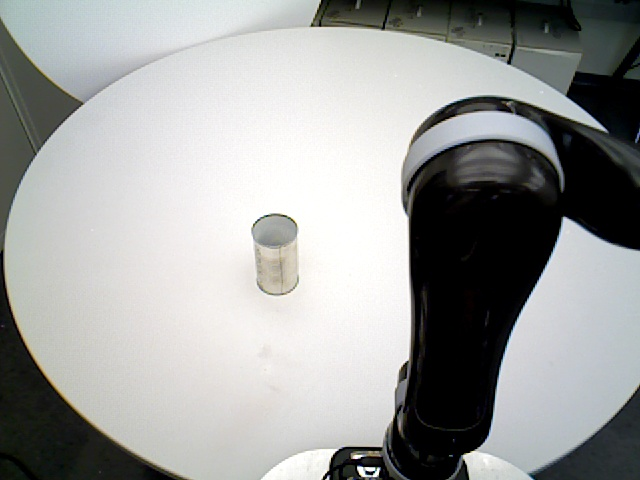
\includegraphics[scale=\examplepicsize]{figures/objects/9.JPG} & 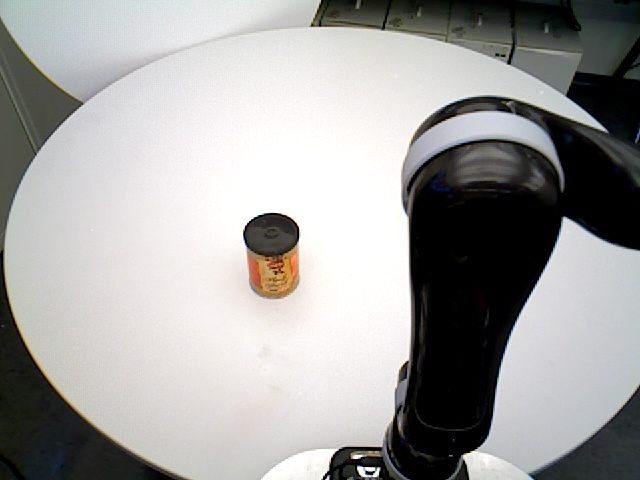
\includegraphics[scale=\examplepicsize]{figures/objects/3.JPG} & 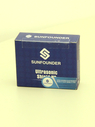
\includegraphics[scale=\examplepicsize]{figures/objects/6.JPG} & 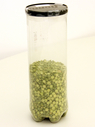
\includegraphics[scale=\examplepicsize]{figures/objects/28.JPG} & 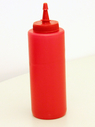
\includegraphics[scale=\examplepicsize]{figures/objects/21.JPG} & 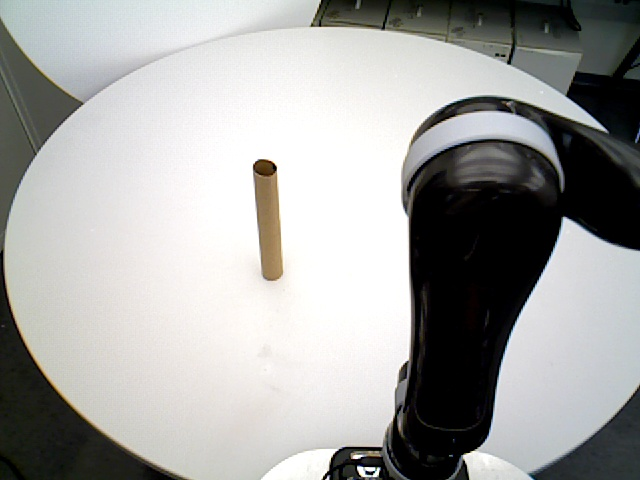
\includegraphics[scale=\examplepicsize]{figures/objects/4.JPG}\\ \hline
	tub & 1 & 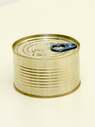
\includegraphics[scale=\examplepicsize]{figures/objects/30.JPG} & 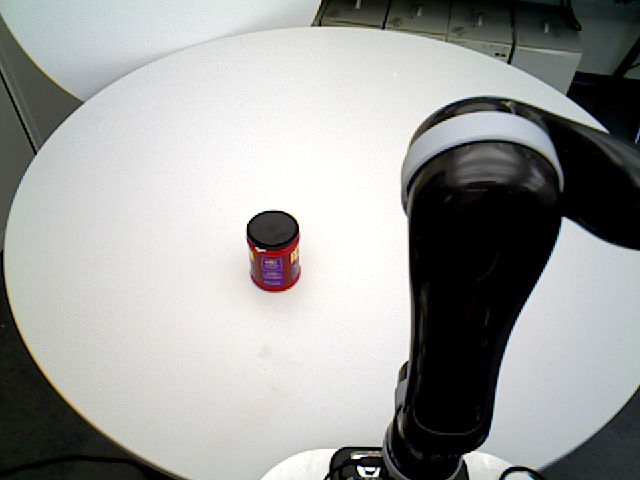
\includegraphics[scale=\examplepicsize]{figures/objects/10.JPG} & 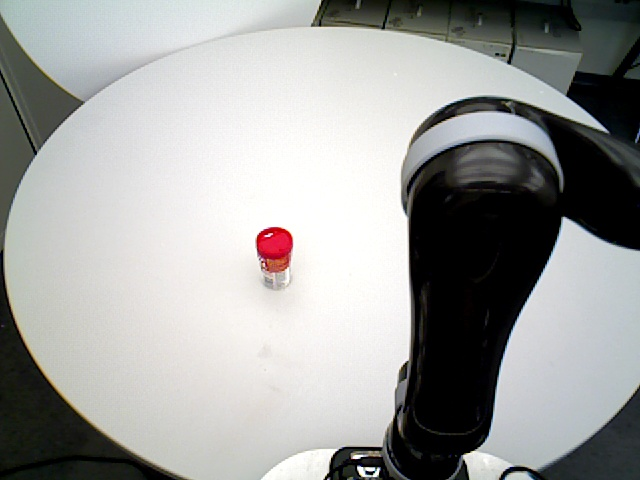
\includegraphics[scale=\examplepicsize]{figures/objects/11.JPG} & 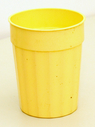
\includegraphics[scale=\examplepicsize]{figures/objects/14.JPG} & 
\includegraphics[scale=\examplepicsize]{figures/objects/2.JPG} & 
\includegraphics[scale=\examplepicsize]{figures/objects/18.JPG}\\ \hline
	empty & .637 & 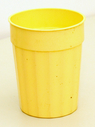
\includegraphics[scale=\examplepicsize]{figures/objects/14.JPG} & 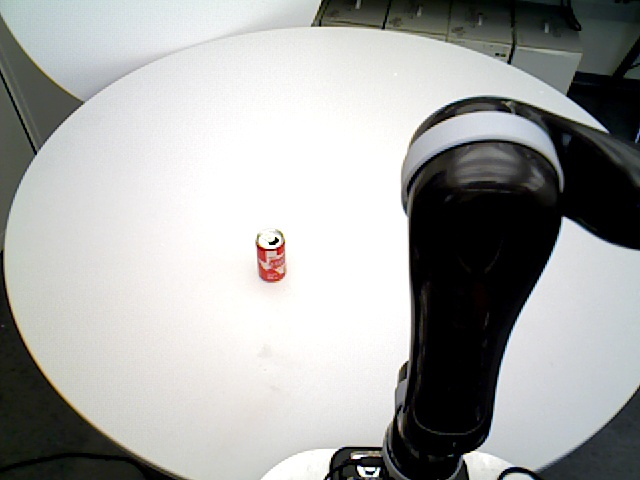
\includegraphics[scale=\examplepicsize]{figures/objects/27.JPG} & 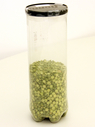
\includegraphics[scale=\examplepicsize]{figures/objects/28.JPG} & 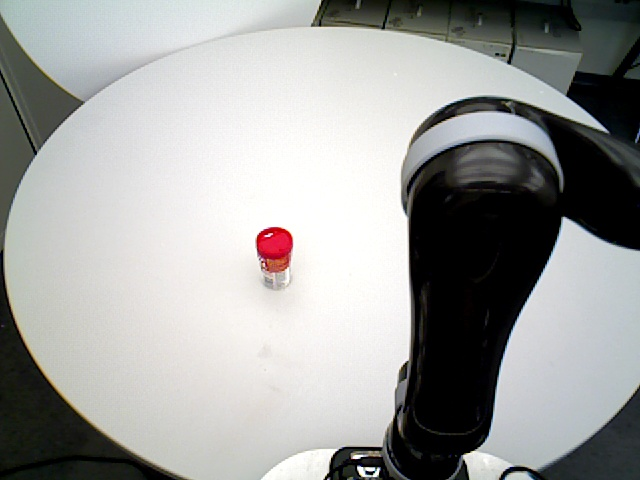
\includegraphics[scale=\examplepicsize]{figures/objects/11.JPG} & 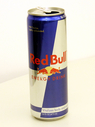
\includegraphics[scale=\examplepicsize]{figures/objects/31.JPG} & 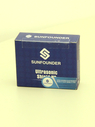
\includegraphics[scale=\examplepicsize]{figures/objects/6.JPG}\\ \hline
	tall & .566 & 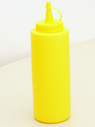
\includegraphics[scale=\examplepicsize]{figures/objects/19.JPG} & 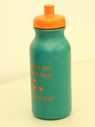
\includegraphics[scale=\examplepicsize]{figures/objects/24.JPG} & 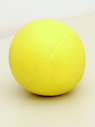
\includegraphics[scale=\examplepicsize]{figures/objects/25.JPG} & 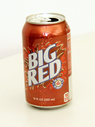
\includegraphics[scale=\examplepicsize]{figures/objects/15.JPG} & 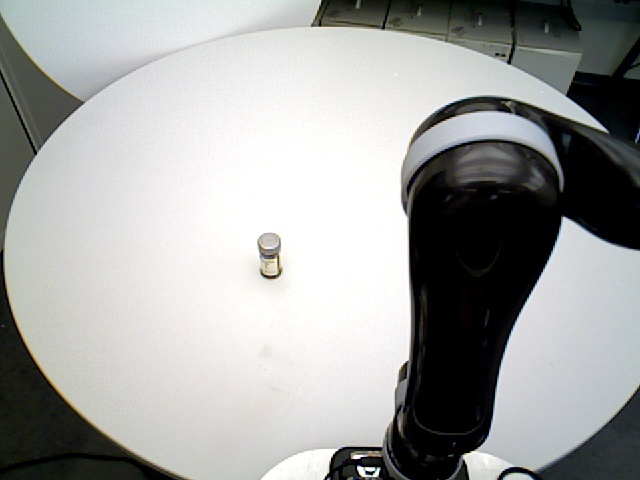
\includegraphics[scale=\examplepicsize]{figures/objects/26.JPG} & 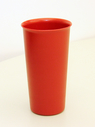
\includegraphics[scale=\examplepicsize]{figures/objects/7.JPG}\\ \hline
	\multicolumn{2}{|c|}{} & \multicolumn{6}{c|}{\bf vision only system} \\ \hline
	small & -.25 & 
\includegraphics[scale=\examplepicsize]{figures/objects/2.JPG} & 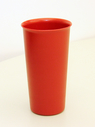
\includegraphics[scale=\examplepicsize]{figures/objects/7.JPG} & 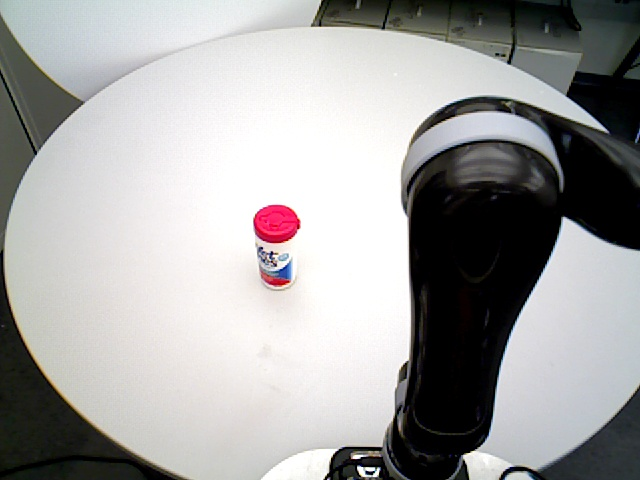
\includegraphics[scale=\examplepicsize]{figures/objects/13.JPG} & 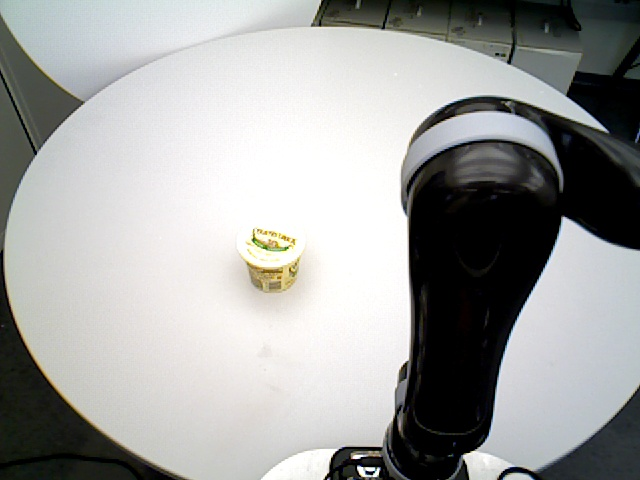
\includegraphics[scale=\examplepicsize]{figures/objects/32.JPG} & 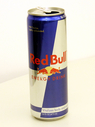
\includegraphics[scale=\examplepicsize]{figures/objects/31.JPG} & 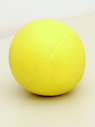
\includegraphics[scale=\examplepicsize]{figures/objects/25.JPG}\\ \hline
	red & -.663 & 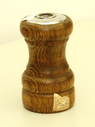
\includegraphics[scale=\examplepicsize]{figures/objects/8.JPG} & 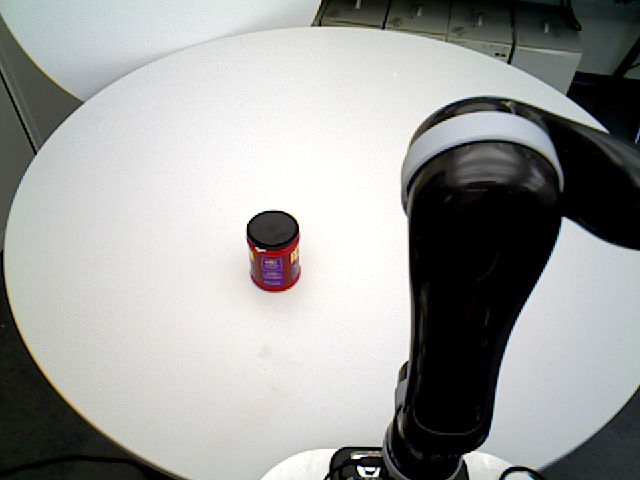
\includegraphics[scale=\examplepicsize]{figures/objects/10.JPG} & 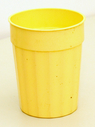
\includegraphics[scale=\examplepicsize]{figures/objects/14.JPG} & 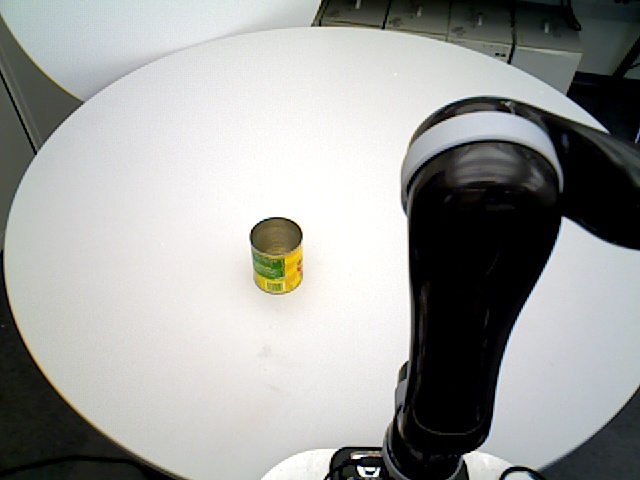
\includegraphics[scale=\examplepicsize]{figures/objects/12.JPG} & 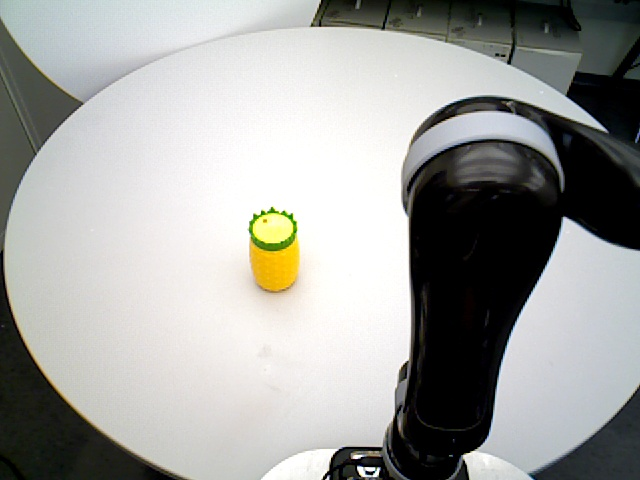
\includegraphics[scale=\examplepicsize]{figures/objects/5.JPG} & 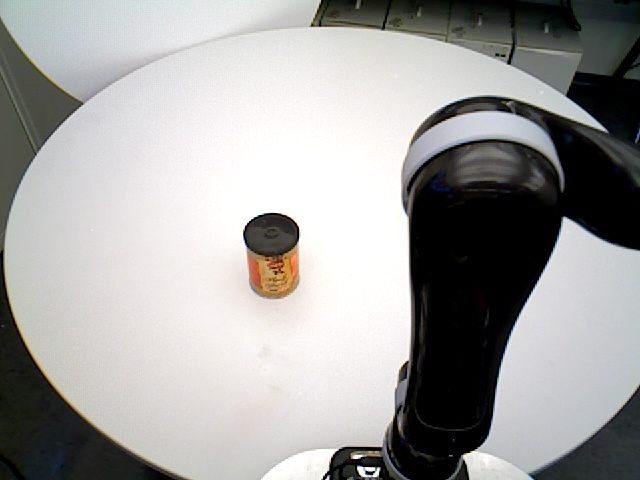
\includegraphics[scale=\examplepicsize]{figures/objects/3.JPG}\\ \hline
	yellow & -1 & 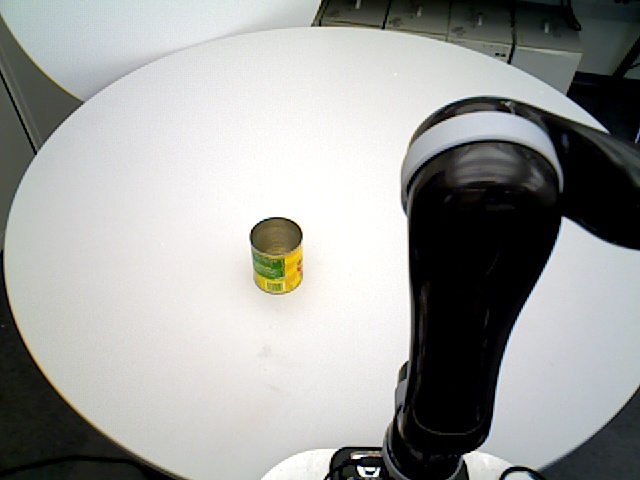
\includegraphics[scale=\examplepicsize]{figures/objects/12.JPG} & 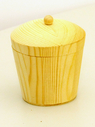
\includegraphics[scale=\examplepicsize]{figures/objects/20.JPG} & 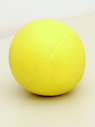
\includegraphics[scale=\examplepicsize]{figures/objects/25.JPG} & 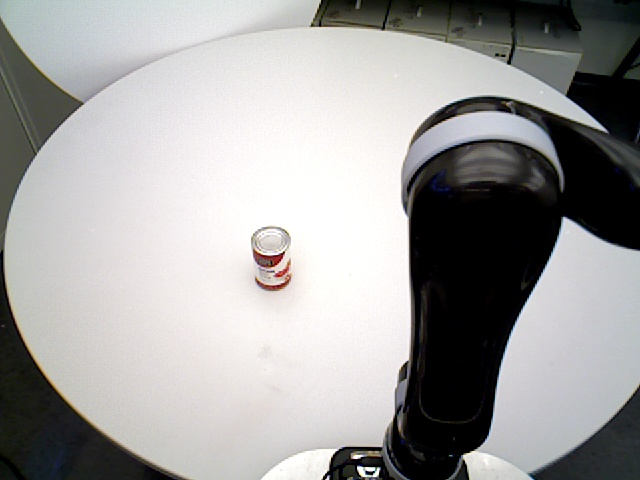
\includegraphics[scale=\examplepicsize]{figures/objects/1.JPG} & 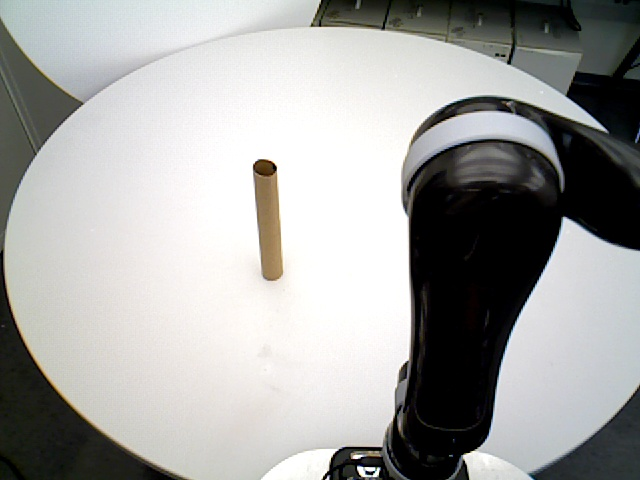
\includegraphics[scale=\examplepicsize]{figures/objects/4.JPG} & 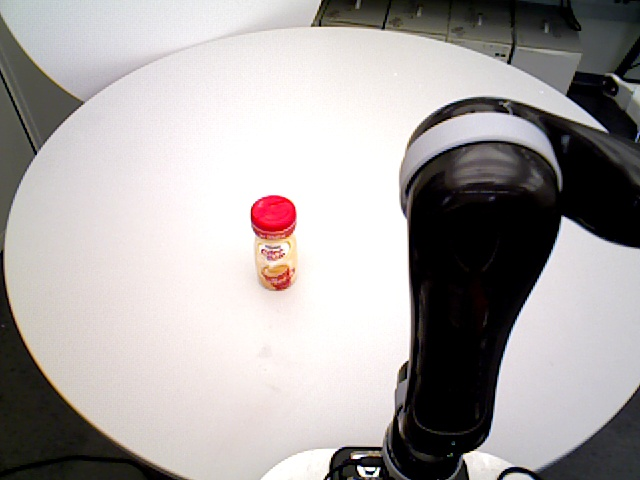
\includegraphics[scale=\examplepicsize]{figures/objects/17.JPG}\\ \hline
\end{tabular}
\caption{Predicates for which the difference $|\kappa_{mm}-\kappa_{vo}|$ between the \textbf{multi-modal} (mm) and \textbf{vision only} (vo) systems was greater than $0.5$ and both systems had at least $10$ objects with labels for that predicate on which to train.}
\label{tab:predicate_examples}
\end{table*}

The \textbf{multi-modal} system achieves total aggrement with human labels for ``can'' and ``tub;''
whereas the \textbf{vision only} system classified all objects as not having these properties, a decision that gives $\kappa=0$.
Something similar happens for the color predicate ``yellow,'' where the \textbf{multi-modal} system classified all objects as yellow, also giving $\kappa=0$.
We note that ``can'' and ``tub'' are cases of category recognition, for which visual data is certainly helpful, but the non-visual attributes of an object can also help (e.g. cans are light, tubs are heavy).
In contrast, ``yellow'' is a color word for which only visual properties are relevant, and the additional noise from other features were enough to confuse the \textbf{multi-modal} approach.

More interesting cases lie between, where non-trivial classifier decisions were made.
The predicates ``empty'' and ``tall'' have non-visual interpretations.
An empty object will be light, while a tall object will exert force earlier against an arm pressing down on it.
The color predicate ``red'' follows the same reasoning as ``yellow'', where non-visual information can serve only to confuse a multi-modal grounding system.
The correlation results in Table~\ref{tab:predicate_correlations} indicate that the \textbf{visiion only} system learned to associate ``small'' with decreased object width, while the \textbf{multi-modal} system was again confused by additional non-visual information.

\paragraph{Correlations to objective measures.}
To validate whether the systems are learning non-visual properties of objects, for every predicate we calculated the Pearson's correlation $r$ between its signed confidence and that object's measured weight, height, and width. Table~\ref{tab:predicate_correlations} gives the correlations with both high coefficient $r$ and high statistical confidence.

\begin{table}
\centering
\begin{tabular}[h]{|l|r|r|}
	\hline
	\bf Property & \bf multi-modal & \bf vision only \\ \hline \hline
	& \multicolumn{2}{c|}{\bf Believable} \\ \hline
	\bf height & tall (.739) & heavy (.729) \\ \hline
	\bf width & fat (.509) & small (-.525) \\ \hline
	\bf weight & empty (-.771) & \\ \hline \hline
	& \multicolumn{2}{c|}{\bf Likely spurious} \\ \hline
	\bf width & & rattles \\ \hline
	& water, blue & \\
	\bf weight & silver, liquid & \\ 
	& gray, red, yellow & \\ \hline
\end{tabular}
\caption{Predicates and associated Pearson's correlation coefficient $r$ between systems' object decisions and physical object properties.
Shown here are predicates for which $r>0.5$ with $p<0.05$ and the system had at least $10$ objects with labels for the predicate on which to train.}
\label{tab:predicate_correlations}
\end{table}

The \textbf{vision only} system seems able to ground ``heavy'' in height and ``small'' in width. the latter of which is a visual word-property pair (``heavy'' for height has counter-examples in our dataset).
The system can represent these shape properties with the vision features associated with the pointcloud.

In contrast, the \textbf{multi-modal} system learned to ground predicates which correlate well to each of the physical dimensions along which we measured objects.
The ``tall'' predicate correlates with objects that are higher, ``fat'' with objects that are wider, and ``empty'' with objects that are lighter.
This highlights the value of multi-modal grounding, since words like ``empty'' cannot be evaluated with vision alone when dealing with closed containers that have unobservable contents.
